% !TeX spellcheck = hu_HU
\documentclass[12pt,a4paper]{article}
\usepackage[utf8]{inputenc}
\usepackage{cmap}
\usepackage[T1]{fontenc}
\usepackage[magyar]{babel}
\usepackage{amsmath}
\usepackage{amsfonts}
\usepackage{amssymb}
\usepackage{graphicx}

\usepackage{outlines}
\usepackage{hyperref}

\hyphenpenalty=10000

\begin{document}

\begin{center}
	\huge
	Valószínűségszámítás és statisztika\\
	\vspace{1mm}
	\LARGE
	Valószínűségszámítás témakör jegyzet\\
	\vspace{5mm}
	\large
	Készült Zempléni András előadásai\\
	és Kovács Ágnes gyakorlatai alapján\\
	\vspace{5mm}
	Sárközi Gergő, 2021-22-2. félév\\
	Nincsen lektorálva!
\end{center}

\tableofcontents

\pagebreak

\section{Előadás 1: Bevezetés}

\subsection{Alapfogalmak}

\begin{outline}
	\1 Eseménytér: $\Omega$, összes lehetséges eredmény (elemi események összessége)
		\2 Elemi esemény: $\omega$, egy lehetséges kimenet
		\2 $\Omega$ részhalmazai: események
		\2 Esemény akkor következik be, ha az egyik elemi eseménye bekötvetkezik
	\1 Esemény: $\Omega$ részhalmaza
		\2 Speciális események: $\Omega$ (biztos), $\emptyset$ (lehetetlen)
		\2 Események összessége: $\mathcal{A}$ (halmazrendszer $\Omega$ részhalmazaiból)
	\1 Műveletek eseményekkel = logikai műveletek = halmazműveletek
		\2 $A \cup B$: vagy (egyik vagy másik vagy mindkettő)
		\2 $A \cap B$: és (mindkettő)
		\2 $\overline{A}$, $A^C$: ellentett, komplementer
	\1 Tulajdonságok:
		\2 $A \setminus B = A \cap \overline{B}$
		\2 De Morgan: $\overline{A \cup B} = \overline{A} \cap \overline{B}$
		\2 $\overline{\overline{A}} = A$, $\overline{\Omega} = \emptyset$
\end{outline}

\pagebreak

\subsection{Valószínűség}

\begin{outline}
	\1 Valószínűség: végtelen próba esetén a relatív gyakoriság
	\1 $A$ valószínűségének jele: $P(A)$ \; ($P(A) \ge 0$, $P(\Omega) = 1$, $P(\emptyset) = 0$)
	\1 Tulajdonságok:
		\2 Egymást kizáró események esetén additív:\\
		$A \cap B = \emptyset \implies P(A \cup B) = P(A) + P(B)$
		\2 $P(A \setminus B) = P(A) - P(A \cap B)$
		\2 $P(A \cup B) = P(A) + P(B) - P(A \cap B)$
	\1 $A$ és $B$ független, ha $P(A \cap B) = P(A) * P(B)$
\end{outline}

\subsubsection{Valószínűségi mező}

\begin{outline}
	\1 Véges valószínűségi mező:
		\2 $\Omega = \{\omega_1, \omega_2, ..., \omega_n\}$
		\2 $p_i = P(\omega_i)$
		\2 $P(A) = P(\bigcup_{\omega_i \in A} \omega_i) = \sum_{\omega_i \in A} p_i$
	\1 Klasszikus valószínűségi mező:
		\2 $p_i = \frac{1}{n}$ (azonos valószínűségű elemi események)
		\2 $P(A) = \frac{k}{n}$ ahol $k$ az $A$ eseményszáma
		\2 Azaz $P(A) = \frac{\text{Kedvező esetek száma}}{\text{Összes eset száma}}$
\end{outline}

\subsubsection{Mintavétel}

\begin{outline}
	\1 $N$ termékből $M$ selejtes, $n$ elemű a minta
	\1 $A$: pontosan $k$ selejtes van a mintában
	\1 Visszatevéses mintavétel:
		\2 $P(A) = {n \choose k} (\frac{M}{N})^k (1 - \frac{M}{N})^{n-k}$
		\2 Ha $p=\frac{M}{N}$: $P(A) = {n \choose k} p^k (1 - p)^{n-k}$
	\1 Visszatevés nélküli mintavétel:
		\2 $P(A) = {M \choose k} {N - M \choose n - k} \; / \; {N \choose n}$
\end{outline}

\pagebreak

\subsubsection{Feltételes valószínűség}

\begin{outline}
	\1 $A$ esemény valószínűségét keressük; tudjuk, hogy $B$ bekövetkezett
	\1 Relatív gyakorisággal: $r_{A \cap B} \; / \; r_B$
	\1 $P(A|B) = \frac{P(A \cap B)}{P(B)}$ ahol $P(B) > 0$
	\1 $P(A|B)P(B) = P(A,B)$ \;\;($A$ és $B$)
\end{outline}

\subsubsection{Teljes eseményrendszer; tételek}

\begin{outline}
	\1 Teljes eseményrendszer: események halmaza, melyek egymást páronként kizárják és egyesítésük $\Omega$.
		\2 $P(A_1) + P(A_2) + ... = 1$
	\1 Teljes valószínűség tétele:
		\2 Legyen pozitív valószínűségű $B_1,B_2,...$ teljes eseményrendszer
		\2 Legyen $A$ tetszőleges esemény
		\2 Ekkor $P(A) = P(A|B_1)P(B_1) + P(A|B_2)P(B_2)+...$
	\1 Bayes tétel:
		\2 Legyen pozitív valószínűségű $B_1,B_2,...$ teljes eseményrendszer
		\2 Legyen $A$ tetszőleges pozitív valószínűségű esemény
		\2 $P(B_k|A) = \frac{P(A|B_k)P(B_k)}{\sum P(A|B_i)P(B_i)} = \text{(magyarázat)} = \frac{P(A \cap B_k)}{P(A)}$
		\2 Komplementerrel: $P(B|A) = \frac{P(A|B)P(B)}{P(A|B)P(B) + P(A|\overline{B})P(\overline{B})}$
\end{outline}

\subsection{Permutáció, variáció, kombináció}

\begin{outline}
	\1 Permutáció: $n$ elem lehetséges sorrendje
	\1 Kombináció (sorrend nem számít) és variáció (sorrend számít):\\
	$n$ elemből $k$ kiválasztása
\end{outline}

\begin{table}[h!]
	\centering
	\begin{tabular}{|c|c|c|c|}
		\hline
		- & Permutáció & Kombináció & Variáció \\
		\hline
		Ismétlés nélkül & $n!$ & ${n \choose k} = \frac{n!}{k!(n-k)!}$ & $\frac{n!}{(n-k)!}$ \\
		\hline
		Ismétléssel & \vtop{\hbox{\strut $k_i$ db egyezik:}\hbox{\strut $\frac{n!}{k_1!*...*k_r!}$}} & ${n + k -1 \choose k}$ & $n^k$ \\
		\hline
	\end{tabular}
\end{table}

\pagebreak

\section{Előadás 2, 3: valószínűségi változók, eloszlások}

\subsection{Események függetlensége}

\begin{outline}
	\1 Nem összekeverni az egymást kizáró eseményekkel!
	\1 $A$ és $B$ események függetlenek, ha $P(A \cap B) = P(A)*P(B)$
	\1 Ha $A$ és $B$ függetlenek, akkor komplementereik is függetlenek
	\1 Ha $A$ és $B$ diszjunktak, akkor csak triviális esetben függetlenek (P=0)
	\1 Önmaguktól csak triviális események függetlenek
	\1 Több páronkénti függetlenségből nem következik összevont függetlenség
	\1 $A \subset B \implies$ csak akkor függetlenek, ha legalább az egyik triviális
	\1 Példa függetlenségre: $A$ az első, $B$ a második kísérlet eredménye
\end{outline}

\subsection{Valószínűségi változók}

\begin{outline}
	\1 Számot rendel egy kísérlet eredményéhez (elemi eseményhez)
	\1 $X:\Omega \to \mathbb{R}$ függvény, hogy $\forall a: \{\omega | X(\omega) < a\} \in \mathcal{A}$
	\1 Eloszlásfüggvény: $F_X(x) = P(X < x)$
		\2 monoton növekvő, balról folytonos
		\2 $\lim\limits_{x \to -\infty} F_X(x) = 0$ és $\lim\limits_{x \to +\infty} F_X(x)=1$ \;\; (tehát $0 \le F_X(x) \le 1$)
	\1 $P(a \le X < b) = F_X(b) - F_X(a)$\\
	$P(a < X \le b) = F_X(b+0) - F_X(a+0)$%\\
	%$P(a < X < b) = F_X(b) - F_X(a+0)$\\
	%$P(a \le X \le b) = F_X(b+0) - F_X(a)$
	\1 Indikátorváltozó eloszlásfüggvénye: $F_X(x) = \begin{cases}
		0, &\text{ha } x \le 0\\
		1-p, &\text{ha } 0 < x \le 1\\
		1, &\text{ha } 1 < x\\
	\end{cases}$
	\1 $X$ folytonos eloszlású, ha eloszlásfüggvénye folytonos, pl:\\
	Egyenletes eloszlás $[a,b]$ intervallumon: $F_X(x) = \begin{cases}
		0, &\text{ha } x \le a\\
		\frac{x-a}{b-a}, &\text{ha } a < x \le b\\
		1, &\text{ha } b < x\\
	\end{cases}$
	\1 Exponenciális eloszlás ($\lambda$ paraméter): $F_X(x) = \begin{cases}
		0, &\text{ha } x \le 0\\
		1-e^{-\lambda x}, &\text{ha } 0 < x
	\end{cases}$
\end{outline}

\pagebreak

\subsubsection{Várható érték, szórás}

\begin{outline}
	\1 Legyen $X:\Omega \to \mathbb{R}$ valószínűségi változó
	\1 Várható érték (mean): $E(X)=EX=\int_\Omega XdP$
	\1 Szórásnégyzet (variance): $D^2(X) = E[(X-EX)]^2=E(X^2)-E^2(X)$
		\2 Átrendezve: $E(X^2) = D^2(X) + E^2(X)$
	\1 Szórás (standard deviation, $\sigma$): $D(X)=\sqrt{D^2(X)}$
	\1 Várható érték lehet végtelen:\\
	$P(X=2^k)=(1/2)^k \implies E(X)=1+1+1+...=\infty$
	\1 Legyen $E(X)$ és $E(Y)$ véges és $a,b \in \mathbb{R}$
		\2 Ekkor $E(aX+b) = aEX+b$
		\2 Ekkor $E(X+Y) = EX+EY$
	\1 $X \ge 0$ és $E(X)$ véges $\implies E(X) \ge 0$
	\1 $D^2(aX+b) = a^2D^2(X)$ \;\; (Tehát $D(aX) = |a|D(X)$)
	\1 $D^2(X+Y) = D^2(X)+D^2(Y)+2cov(X,Y)$
	\1 Ha $X$ nemnegatív egész értékű: $E(X) = P(X\ge1) + P(X\ge2) + ...$
		\2 pl. dobókocka: $E(X)=3.5=\frac{6}{6}+\frac{5}{6}+\frac{4}{6}+\frac{3}{6}+\frac{2}{6}+\frac{1}{6}$
	\1 Attól még, hogy $E(X)$ véges, $D^2(X)$ nem feltétlenül véges:\\
	pl.: $P(X=k)=c/k^3$ ha eloszlás, attól még $E(X^2)=c(1/1+1/2+...)$
	\1 $X$, $Y$ függetlenek $\implies E(XY)=E(X)E(Y)$
	\1 $Z$: $p$ valószínűséggel $X$, $1-p$ valószínűséggel $Y$:\\
	$E(Z) = p*E(X) + (1-p)*E(Y)$
\end{outline}

\subsubsection{Valószínűségi változó: egyebek}

\begin{outline}
	\1 Vektor valószínűségi változó: ha $\underline{X}$ koordinátái függetlenek:\\
	$F_{\underline{X}}(\underline{z}) = P(X_1 < z_1, X_2 < z_2, ...) = F_1(z_1)F_2(z_2)...$
	\1 $iid$ ($i.i.d.$) jelentése: független és azonos eloszlású
\end{outline}

\pagebreak

\subsection{Diszkrét valószínűségi változók}

\begin{outline}
	\1 Értékkészlet véges vagy megszámlálhatóan végtelen
		\2 Véges, vagy megszámlálhatóan végtelen valószínűségi mezőn minden valószínűségi változó diszkrét
	\1 Legyen $X=(x_1,...,x_n)$, ekkor $p_i = P(X = x_i)$ és $\sum_{i=1}^{n} P(X=x_i) = 1$
	\1 Elfajult eloszlás: $\forall \omega: X(\omega) = c$,\; $P(X=c)=1$
	\1 Ha $X$ diszkrét valószínűségi változó: $\{\omega | X(\omega)=x_i\}$ teljes eseményrendszer
	\1 $X+Y$, mint diszkrét valószínűségi változó
		\2 $P(X+Y=z)=\sum_y P(X=z-y,\; Y=y)$
		\2 Ha $X$ és $Y$ függetlenek:\\
		$P(X+Y=z) = \sum_{x_i+y_j=z} P(X=x_i)P(Y=y_j)$
\end{outline}

\subsubsection{Valószínűségi változók függetlensége}

\begin{outline}
	\1 $X$ és $Y$ függetlenek, ha $\forall i,k:$\\
	$P(\{X=x_i\} \cap \{Y = Y_k\}) = P(X=x_i)*P(Y=y_k)$
		\2 (Azaz, ha $X$-hez és $Y$-hoz tartozó teljes eseményrendszerek függetlenek)
	\1 Elfajult eloszlású valószínűségi változó miden val. változótól független
	\1 Önmagától csak az elfajult eloszlású valószínűségi változó független
\end{outline}

\subsubsection{Várható érték, szórás}

\begin{outline}
	\1 $E(X)=\sum x_k P(X=x_k)$ ha a végtelen összeg abszolút konvergens
		\2 $E(X^2)$: az $x_k$ értéket négyzetre kell emelni
		\2 Dobókocka: $E(X)= \frac{1}{6}*\sum_{i=1}^{6} i = 3.5$\\
		És a szórásnégyzet: $D^2(X)=91/6 - 3.5^2 = 105/36$
	\1 Elfajult eloszlás várható értéke: $E(X)=cP(X=c)=c$
	\1 Egyenletes eloszlás várható értéke: számok számtani közepe
	\1 Függvény várható értéke: $E(g(x)) = \sum P(X=x_i) g(x_i)$
\end{outline}

\pagebreak

\subsubsection{Nevezetes diszkrét eloszlások}

\begin{figure}[h!]
	\centering
	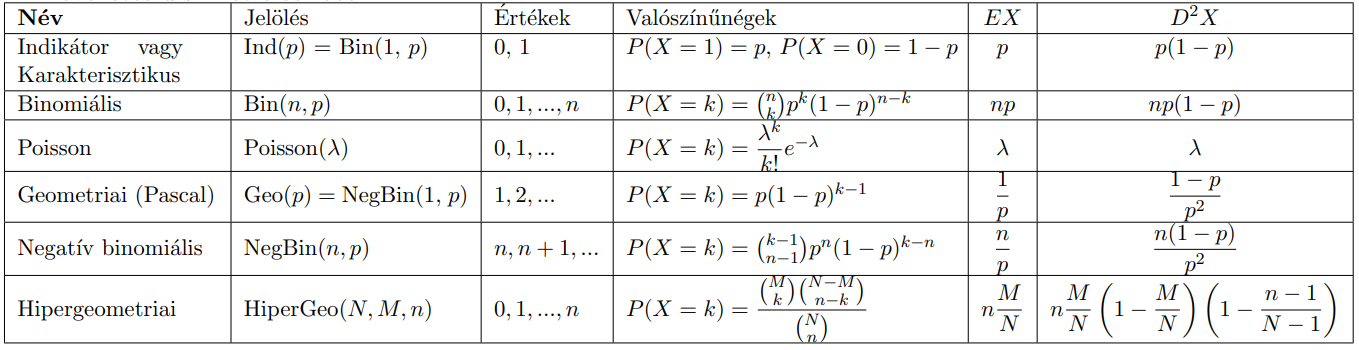
\includegraphics[width=1\linewidth]{diszkrét-eloszlások}
\end{figure}

\begin{outline}
	\1 Indikátor: $p$ valószínűségű esemény bekövetkezik-e vagy sem
	\1 Binomiális: visszatevéses mintavétel
	\1 Poisson: időben lejátszódó folyamatnál adott $[a,b)$ intervallumba eső események száma ($X_{a,b}$) éppen $\lambda(b-a)$ paraméterű Poisson eloszlású
		\2 ha homogén az esemény: $\lambda$ nem változik az idővel
		\2 ha utóhatás nélküli az esemény: a<b<c $\implies X_{a,b}$ és $X_{b,c}$ függetlenek
		\2 nemelfajuló: $0 < P(X_{a,b}=0) < 1$
	\1 Geometriai (Pascal): hányadikra következik be először egy $p$ valószínűségű
	\1 Negatív binomiális: hányadikra következik be $n$. alkalommal egy $p$ valószínűségű esemény
	\1 Hipergeometriai: visszatevés nélküli mintavétel
\end{outline}

\subsection{Gyakorlat}

\begin{outline}
	\1 Diszkrét eloszlást a $P(X=...)=...$ értékekkel adhatjuk meg
\end{outline}

\pagebreak

\section{Előadás 3: kovariancia, korreláció}

\subsection{Kovariancia}

\begin{outline}
	\1 $cov(X,Y) = E(\; (X-E(X))*(Y-E(Y)) \;) =$\\
	$=E(\; XY - XE(Y) - YE(X) - E(X)E(Y) \;) =$\\
	$=E(XY) - E(X)E(Y)$
	\1 $X,Y$ függetlenek $\implies cov(X,Y) = 0$ \;\; (Visszafelé nem igaz)
	\1 Szimmetrikus: $cov(X,Y)=cov(Y,X)$
	\1 Kapcsolat szórásnégyzethez: $cov(X,X) = D^2(X)$
	\1 Skálafüggő: $cov(a*X, b*Y) = ab*cov(X,Y)$
\end{outline}

\subsection{Korrelációs együttható}

\begin{outline}
	\1 Változók közötti lineáris kapcsolat erősségét méri:\\
	$R^2 \approx 1$ az erős kapcsolatot, $R^2 \approx 0$ a gyenge kapcsolatot jelenti
	\1 $R(X,Y) = \frac{cov(X,Y)}{D(X)D(Y)}$
	\1 $X,Y$ függetlenek $\implies R(X,Y) = 0$ \;\; (Visszafelé nem igaz)
	\1 $X$ vagy $Y$ elfajult $\implies R(X,Y)=0$
	\1 $R(X,aX+b) = 1$ ha $a>0$
\end{outline}

\pagebreak

\section{Előadás 4: abszolút folytonos eloszlások}

\begin{outline}
	\1 Sűrűségfüggvény eloszlásfüggvényből
		\2 Legyen $F$ eloszlásfüggvény és létezzen $f$, hogy $F(z) = \int_{-\infty}^{z}f(t)dt$
		\2 Ekkor $f$ sűrűségfüggvény és $F$ abszolút folytonos
		\2 $f$ nem egyértelmű $\implies$ legegyszerűbb szakaszonként folytonos változatát vesszük
	\1 Eloszlásfüggvény sűrűségfüggvényből: (fentieken túl)
		\2 Ha $X \ge 0$, akkor $F(0)=0$ (ebből integrálás konstans szerezhető)
	\1 $P(a < X \le b) = P(a \le X < b) = F(b) - F(a)$
	\1 Várható érték: $E(X) = \int_{-\infty}^{+\infty}xf(x)dx$ (ha az integrál létezik)
		\2 Függvény várható értéke: $E(g(x)) = \int_{-\infty}^{+\infty}g(x)f(x)dx$
\end{outline}

\subsection{Sűrűségfüggvény}

\begin{outline}
	\1 Legyen $X$ abszolút folytonos eloszlású
	\1 $f(x) = F'(x)$ (esetleg néhány pont kivételével)
	\1 $f(x) \ge 0$ és $\int_{-\infty}^{+\infty}f(x)dx = 1$
		\2 Megengedett: $\exists x: f(x) > 1$
	\1 $F$ folytonos, tehát $\forall x: P(X=x) = 0$
\end{outline}

\subsection{Standard normális eloszlás}

\begin{outline}
	\1 Sűrűségfüggvény: $f(x) = \frac{1}{\sqrt{2\pi}} e^{-x^2/2}$
		\2 Haranggörbe, csúcs $x=0$-ban
	\1 Normális eloszlás standardizálása:
		\2 Legyen $X \sim N(m, \sigma^2)$
		\2 Ekkor $\frac{X-m}{\sigma} \sim N(0,1)$
\end{outline}

\pagebreak

\subsection{Nevezetes abszolút folytonos eloszlások}

\begin{figure}[h!]
	\centering
	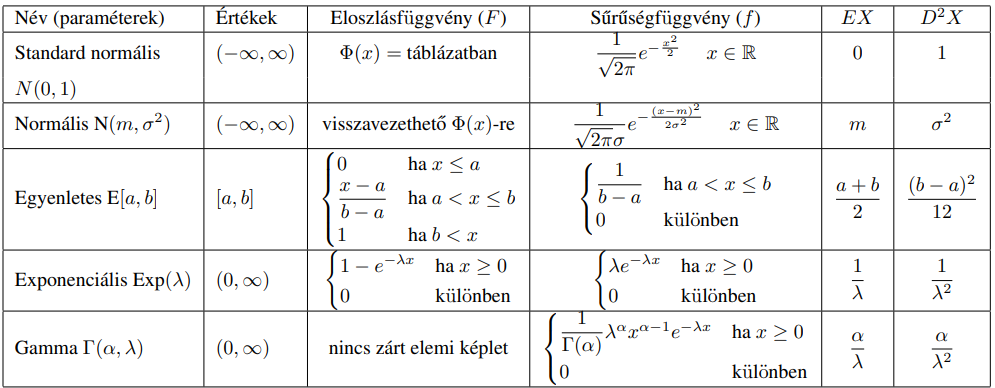
\includegraphics[width=1\linewidth]{abszolút-folytonos-eloszlások}
\end{figure}

\begin{outline}
	\1 A "geometriai modell" az egyenletes eloszlást jelent
	\1 Chi-négyzet eloszlás ($Ki^2$): $X \sim \chi^2_n$ ha $X = \sum Z_i$ ahol $Z_i \sim N(0,1)$
	\1 $t$ eloszlás: $X \sim t_n$ ha $X=\frac{Z}{\sqrt{Y_n/n}}$ ahol $Z \sim N(0,1)$ és $Y_n \sim \chi^2_n$
	\1 $F$ eloszlás: $X \sim F_{n_1,n_2}$ ha $X=\frac{U_1/n_1}{U_2/n_2}$ ahol $U_i \sim \chi^2_{n_i}$
\end{outline}

\subsection{Függvény eloszlása}

\begin{outline}
	\1 $X$ egy valószínűségi változó $\implies$ $g(X)$ is az
	\1 $X$ folytonosságából NEM következik $g(X)$ folytonossága
	\1 Legyen $X$ abszolút folytonos
	\1 Legyen $g : \mathbb{R} \to \mathbb{R}$, folytonosan differenciálható, $g' \ne 0$
	\1 $Y=g(x)$ eloszlásfüggvénye:\\
	$F_Y(y) = F_{g(x)}(y) = \begin{cases}
	F_X(g^{-1}(y)) & \text{ha $g$ szig. mon. nő}\\
	1 - F_X(g^{-1}(y)) & \text{ha $g$ szig. mon. csökken}
	\end{cases}$
		\2 Példa: $F_{aX+b} = F_X((z-b)/a)$ ha $a > 0$
		\2 Példa: $F_{aX+b} = 1 - F_X((z-b)/a)$ ha $a < 0$
	\1 $Y=g(X)$ sűrűségfüggvénye:\\
	$f_Y(y) = f_{g(x)}(y) = F_X(g^{-1}(y)) * |(g^{-1}(y))'| = f_X(g^{-1}(y)) \;/\; |g'(g^{-1}(y))|$\\
	Lényeg: $f_{g(x)}(y) = f_X(g^{-1}(y)) \;/\; |g'(g^{-1}(y))|$
\end{outline}

\pagebreak

\subsection{Együttes eloszlásfüggvények elnevezései}

\begin{outline}
	\1 Együttes eloszlásfüggvény: $F_{X,Y}(x,y) = P(X < x, Y < y)$
	\1 Peremeloszlásfüggvények: $F_X(x) = P(X < x)$, $F_Y(y) = P(Y < y)$
	\1 Együttes sűrűségfüggvény: $f_{X,Y}(x,y)$
	\1 Peremsűrűségfüggvények: $f_X(x)$, $f_Y(y)$
\end{outline}

\subsection{Együttes eloszlásfüggvények kapcsolata}

\begin{outline}
	\1 $F_X(x) = \lim\limits_{y \to \infty} F_{X,Y}(x,y)$
	\1 $F_{X,Y}(x,y) = \int_{-\infty}^{y} \int_{-\infty}^{x} f_{X,Y}(u,v) dudv$
	\1 $f_{X,Y}(x,y) = \partial_y \partial_x F_{X,Y}(x,y) = \partial_x \partial_y F_{X,Y}(x,y)$
	\1 $\int_{-\infty}^{+\infty} \int_{-\infty}^{+\infty} f_{X,Y}(x,y) dxdy = 1$
	\1 $F_X(x) = \int_{-\infty}^{+\infty} f_{X,Y}(x,y)dy$
	\1 $X,Y$ függetlenek $\Leftrightarrow$ $F_{X,Y}(x,y) = F_X(x)*F_Y(y)$
	\1 $X,Y$ függetlenek $\Leftrightarrow$ $f_{X,Y}(x,y) = f_X(x)*f_Y(y)$
	\1 Diszkrét esetben:\\
	$X,Y$ függetlenek $\Leftrightarrow$ $P(X = x, Y = y) = P(X = x) * P(Y = y)$
	\1 $X,Y$ függetlenek $\Leftrightarrow$ $E(XY) = E(X) * E(Y)$
\end{outline}

\section{Előadás 5: máshová írtam be az anyagot}

\pagebreak

\section{Előadás 6: egyenlőtlenségek, aszimptotikus tulajdonságok}

\subsection{Markov-típusú egyenlőtlenségek}

\begin{outline}
	\1 Legyen $X \ge 0$ val. változó, legyen $g : \mathbb{R}_+ \to \mathbb{R}_+$ monoton növő
	\1 Ekkor $\epsilon > 0$ esetén $P(X \ge \epsilon) \le \frac{E(g(X))}{g(\epsilon)}$
	\1 Bizonyítás: $E(g(X)) \ge g(\epsilon)P(X \ge \epsilon)$ mert $X \ge \epsilon \implies g(X) \ge g(\epsilon)$
\end{outline}

\subsubsection{Alkalmazásai}

\begin{outline}
	\1 Gyakorlatban nem kellően pontos becslést adnak, konkrét eloszlás ismeretével pontosabb becslés szerezhető
	\1 Markov egyenlőtlenség:
		\2 $g(x)=x$ és $X \ge 0$ val. változó esete, ekkor $P(X \ge \epsilon) \le \frac{E(X)}{\epsilon}$
		\2 Máshogy: $P(X \ge k*E(X)) \le \frac{E(X)}{k*E(X)} = \frac{1}{k}$
	\1 Csebisev egyenlőtlenség:
		\2 $g(x)=x$ és $X$ helyett $(X-EX)^2$ esete
		\2 $P((X-EX)^2 \ge \epsilon^2) \le \frac{E(X-EX)^2}{\epsilon^2} \; \implies \;$
		$P(|X-EX| \ge \epsilon) \le \frac{D^2(X)}{\epsilon^2}$
\end{outline}

\subsection{Konvergencia típusai}

\begin{outline}
	\1 Legyen $X_i$ val. változók sorozata, ekkor $X_n \to (n \to +\infty) \to X$...
	\1 ... 1 valószínűséggel: $P(\{ \omega \;:\; X_n(\omega) \to (n \to +\infty) \to X(\omega) \}) = 1$
	\1 ... gyengén: ha eloszlásfüggvényeikre $F_n(x) \to (n \to +\infty) F(x)$
		\2 $F$ minden folytonossági pontjában
\end{outline}

\subsection{Nagy számok törvényei}

\begin{outline}
	\1 Legyen $X_1, X_2, ..., X_n$ független, azonos eloszlású valószínűségi változók
	\1 Legyen a várható értékük (ami azonos, hiszen azonos az eloszlás) véges
	\1 $\frac{X_1 + ... + X_n}{n} \to m = E(X_i) = E(X_1)$ ha $n \to +\infty$
	\;\; (1 valószínűséggel)
\end{outline}

\pagebreak

\subsection{Centrális határelosztás tétel}

\begin{outline}
	\1 Legyen $X_1, X_2, ..., X_n$ független, azonos eloszlású valószínűségi változók
	\1 Legyen a szórásnégyzetük ($\sigma^2 = D^2(X_i)$) véges
		\2 Nulla sem lehet, nem? Hiszen osztunk vele
	\1 Szórásuk, várható értékük ($m=E(X_i)$) egyezik, mert azonos az eloszlásuk
	\1 $\frac{X_1 + ... + X_n - n*m}{\sqrt{n} * \sigma} \to N(0,1)$ ha $n \to +\infty$
	\;\; (gyengén)
		\2 Máshogy: $P(\frac{X_1 + ... + X_n - n*m}{\sqrt{n} * \sigma} < x) \to \Phi(x)$
		\2 Máshogy: $n$ kísérlet összegének szórása $\frac{1}{\sqrt{n}}$-nel arányos
	\1 Legyen $\overline{X}$ átlag: $\overline{X} = \frac{X_1 + ... X_n}{n}$,
	ekkor $\overline{X} \sim N(\mu, (\frac{\sigma}{\sqrt{n}})^2)$ \;\; ($E(X_i) = \mu$)
	\1 Felhasználás: $0.9$ valószínűséggel legyen $X < 99.5$ ahol $X \sim N(100, 3^2)$
		\2 $\overline{X} \sim N(100, (\frac{3}{\sqrt{n}})^2)$ a tétel szerint
		\2 Legyen $S$ std normál: $S \sim N(0,1)$
		\2 $0.9 = P(\overline{X} < 99.5) = P(S < \frac{99.5-100}{3/\sqrt{n}}) = \Phi(\frac{99.5-100}{3/\sqrt{n}})$
		\2 Megoldás: $0.9 = \Phi(\frac{99.5-100}{3/\sqrt{n}}) = \Phi(\frac{\sqrt{n}}{-6}) = \Phi(\frac{\sqrt{n}}{6})$\\
		$n=(qnorm(0.9) * 6)^2 \approx 59.12$
\end{outline}

\pagebreak

\section{R jegyzet}

\begin{outline}
	\1 choose(x, y); \verb|cat("X:", x, "\n", "valami"))|; round(x, 4)
	\1 diszkrét
		\2 ppois, pbinom, phyper
		\2 sum(dbinom(0:4, 12, 0.2)) = pbinom(4, 12, 0.2)
		\2 \begin{verbatim}
		barplot(dbinom(0:6, 6, 527/1000),
		        col="red",
		        xlab="k értéke",
		        ylab="Valószínűség",
		        main="Binomiális eloszlás",
		        names.arg = 0:6)
		\end{verbatim}
	\1 abszolút folytonos
		\2 pnorm
		\2 d\{dist\}(a, ...) = f(a)
		\2 p\{dist\}(a, ...) = F(X < a)
		\2 q\{dist\}(p, ...) = a $\implies$ F(X < a) = p
		\2 \begin{verbatim}
		valx <- seq(90, 110, 0.01)
		valy <- pnorm(valx, 100, 2)
		plot(valx, valy, col = "red", type = "l", lwd = 2,
		     xlab = "x", ylab = "Fi(x)",
		     main = "Eloszlásfüggvény")
		abline(h = c(0, 1), lty = 2)
		\end{verbatim}
	\1 plot-olás
		\2 lwd: line width (2-3 szokott lenni)
		\2 lty: line type, (1=folytonos, 2=dashed, 3=dotted, ...)
		\2 \begin{verbatim}
		my_plot <- function(f, from_x, to_x) {
		  x <- seq(from_x, to_x, 1 / 100)
		  y <- sapply(x, f)
		  plot(x, y, type = "l", col = "black", lwd = 3)
		  abline(h = c(0, 1))
		}
		\end{verbatim}
\end{outline}

\end{document}
